\subsection{Conexión i2c}
Para un Paquito, es necesario que su \textbf{arduino} y su \textbf{raspberry pi} estén comunicados entre sí. Necesitamos que la \textbf{raspberry pi} haga cálculos a alto nivel, y que el \textbf{arduino} haga cálculos a un bajo nivel. Para lograr esta comunicación, utilizaremos un protocolo llamado \textbf{i2c}.

Usualmente en una comunicación que utiliza el protocolo \textbf{i2c} sólo necesitas conectar ciertos pines directamente de un dispositivo a otro. Sin embargo, resulta que la raspberry pi y el arduino trabajan con un voltaje de lógica diferente. Por tanto, necesitamos de un pequeño chip conversor en medio de la comunicación i2c para que los dispositivos no se quemen.

\begin{miencuadre}
    El voltaje de lógica (lógica de control) de un dispositivo es la cantidad de voltaje con la que trabaja una placa. Es el rango de tensión eléctrica que representa un cero (0) o un uno (1) en circuitos digitales. [1] La raspberry pi de un Paquito trabaja con una lógica de voltaje de 3.3V (se ocupan 3.3V aproximadamente para representar un 1), mientras que el arduino de un Paquito trabaja con una lógica de voltaje de 5V (se ocupan 5V aproximadamente para representar un 1).
\end{miencuadre}

Este chip conversor que se usa para los paquitos es el \textit{4-Channel Bidirectional Logic Level Converter 5V to 3.3V. (Level Shifter)}, y se puede ver el la figura \ref{fig:level-shifter}. Como se puede ver en la figura \ref{fig:level-shifter}, este chip tiene de un lado marcas que empiezan con \textit{HV}, y de otro lado marcas que empiezan con \textit{LV}. Las letras \textit{HV} significan HIGH VOLTAGE, miestras que las letras \textit{LV} significan LOW VOLTAGE. Del lado de HIGH VOLTAGE se conectará la placa con la lógica de voltaje más alta (el arduino), mientras que del lado de LOW VOLTAGE se conectará la placa con la lógica de voltaje más baja (la raspberry). 

\begin{figure}[htbp]
    \centering
    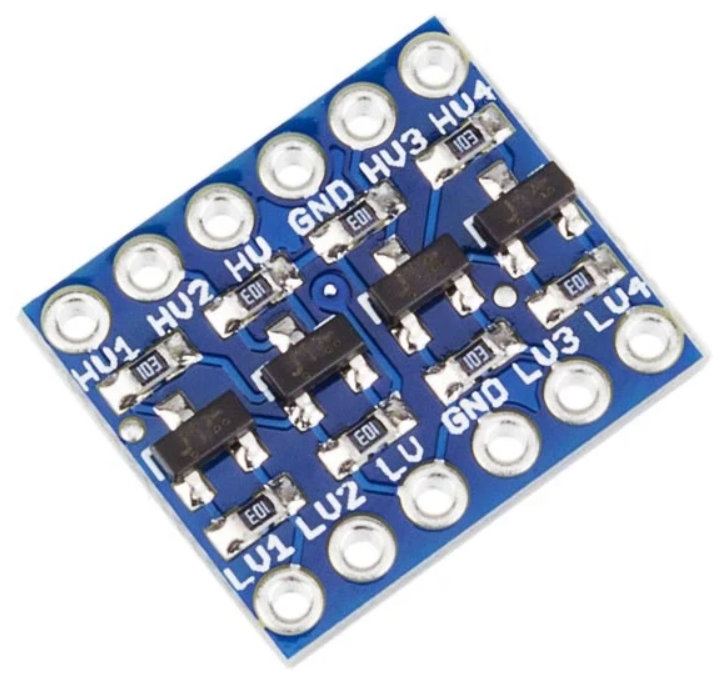
\includegraphics[width=0.5\textwidth]{imagenes/level-shifter.png}
    \caption{Chip conversor para Paquitos.}
    \label{fig:level-shifter}
\end{figure}

Entonces, para iniciar una comunicación i2c, debemos de conectar ambas placas de la siguiente manera:
\begin{enumerate}
    \item Conectar el pin SDA de la raspberry al pin LV1 del chip conversor. Luego conectar el pin HV1 del chip conversor al pin SDA del arduino.
    \item Conectar el pin SCL de la raspberry al pin LV2 del chip conversor. Luego conectar el pin HV2 del chip conversor al pin SCL del arduino.
    \item Conectar un pin GND de la raspberry al pin GND del chip conversor que está del lado de los pines LV. Luego conectar el pin GND del chip conversor que está del lado de los pines HV, a un pin de GND del arduino.
    \item Conectar un pin de 3.3V de la raspberry al pin LV del chip conversor. Luego conectar el pin HV del chip conversor a un pin de 5V del arduino.
\end{enumerate}

Esta conexión se resume en el cuadro \ref{fig:cserial}, y se puede ilustra en la figura \ref{fig:i2c}.

\begin{table}[h]
    \centering
    \begin{tabular}{|c|c|c|c|}
        \hline
        Raspberry Pi & Conversor (LV) & Conversor (HV) & Arduino \\
        \hline
        SDA & LV1 & HV1 & SDA \\
        SCL & LV2 & HV2 & SCL \\
        GND & GND (LV) & GND (HV) & GND \\
        3.3V & LV & HV & 5V \\
        \hline
    \end{tabular}    
    \caption{Conexión Serial.}
    \label{fig:cserial}
\end{table}



\begin{figure}[htbp]
    \centering
    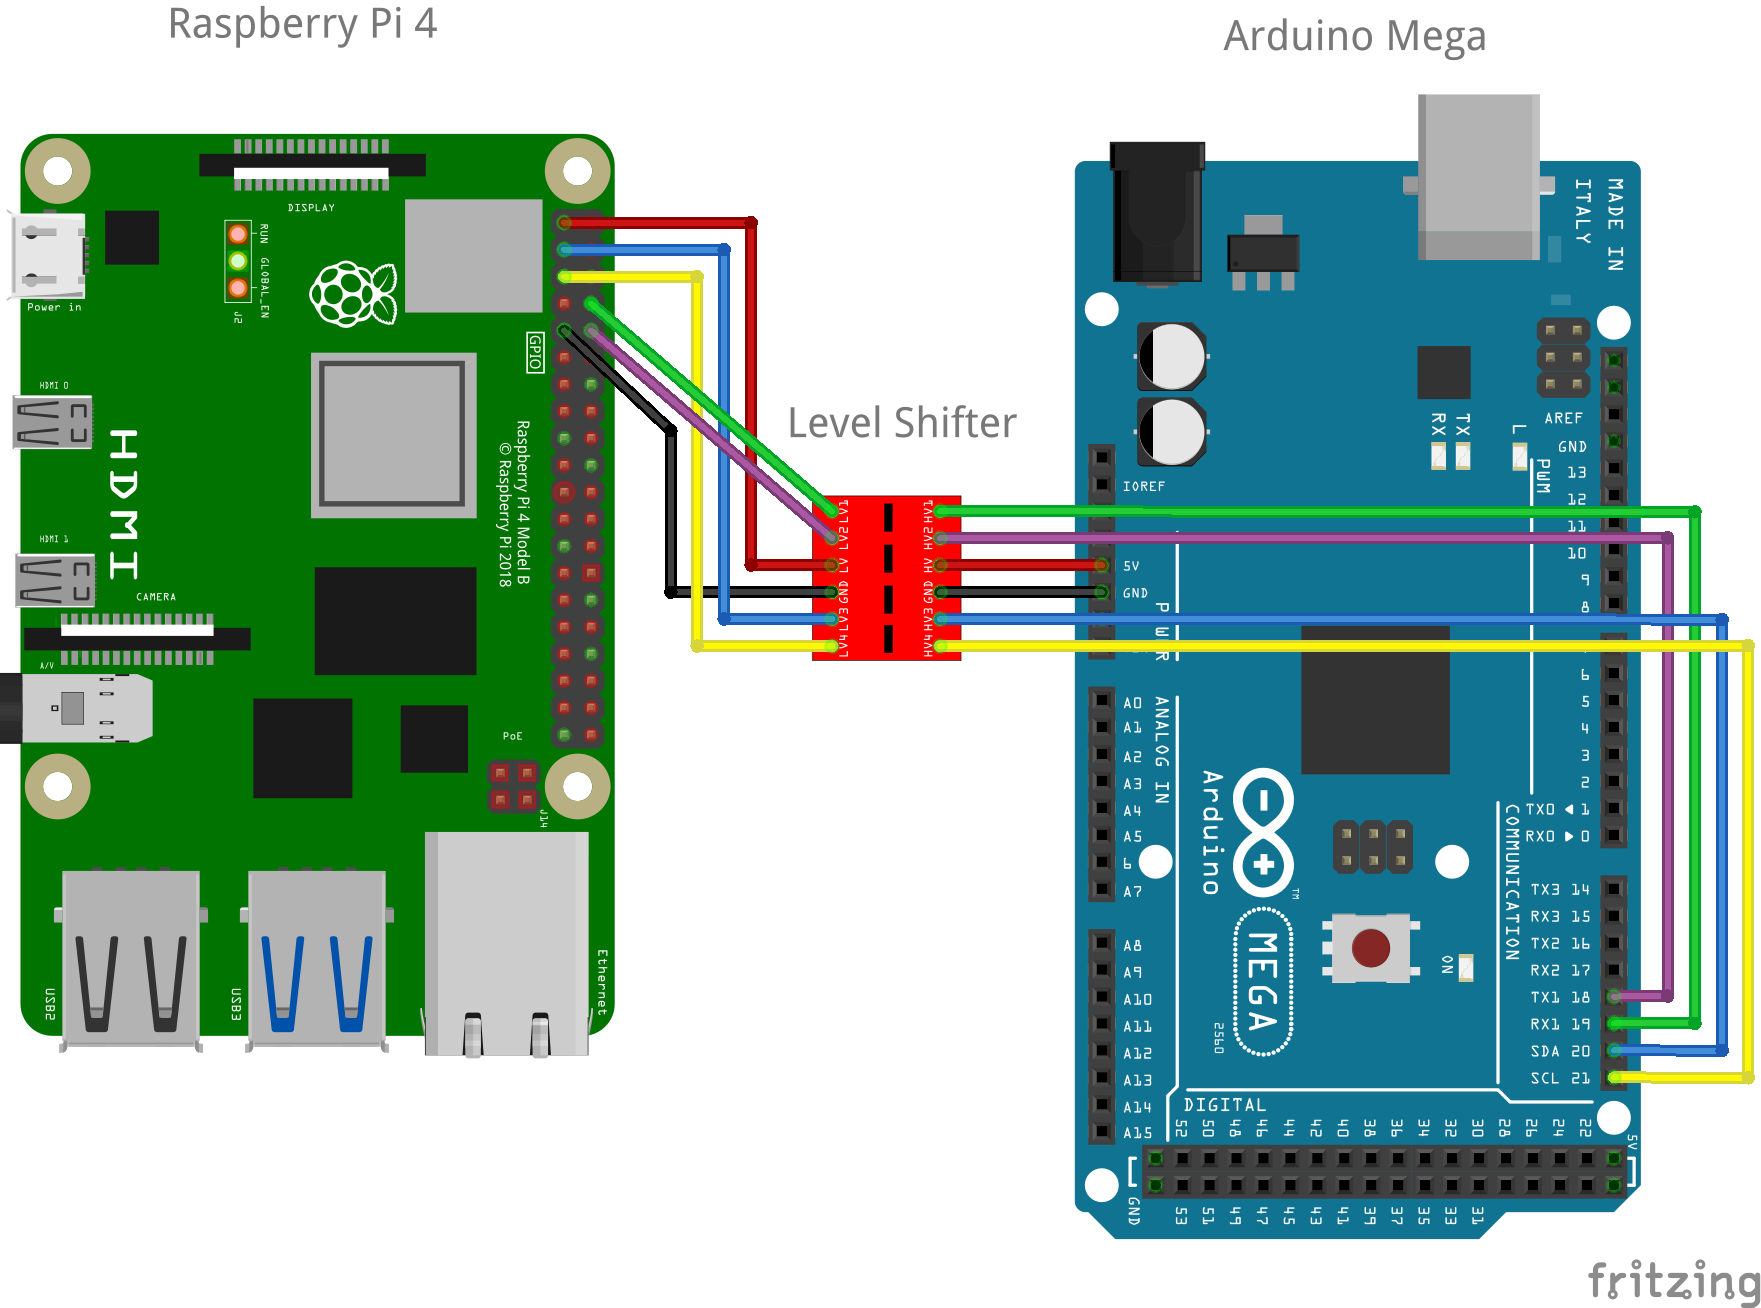
\includegraphics[width=0.7\textwidth]{imagenes/i2c-connection_bb.png}
    \caption{Conexión i2c y serial.}
    \label{fig:i2c}
\end{figure}


